\documentclass[11pt]{article}

\usepackage{url}
\usepackage{multicol}
\usepackage[english]{babel}
\usepackage[margin=1in]{geometry}
\usepackage{graphicx}
\usepackage{subcaption}
\usepackage{enumitem}
\usepackage{amsmath}
\usepackage{amssymb}
\usepackage{wasysym}
\usepackage{color}
\usepackage{float}
\usepackage{nomencl}
\usepackage[title]{appendix}
\makenomenclature
\usepackage{pdfpages}
\usepackage{algorithm}
\usepackage{algpseudocode}
\usepackage{hyperref}
\hypersetup{
    colorlinks=true,
    linkcolor=blue,
    filecolor=magenta,      
    urlcolor=cyan,
    pdftitle={Overleaf Example},
    pdfpagemode=FullScreen,
    }
\title{16-745 Optimal Control Lecture 5}
\author{Reid Graves} 

\begin{document}
\maketitle

\section{Last Time}
\begin{enumerate}
    \item Minimization with equality constraints
\end{enumerate}

\section{Today}
\begin{itemize}
    \item Inequality constraints
\end{itemize}

\section{Inequality Constrained Minimization}
\begin{align*}
    \text{min}_x f(x)
    \\
    s.t. \quad c(x)\geq 0
\end{align*}

\begin{itemize}
    \item KKT conditions:
    \begin{align*}
        \nabla f - \left(\frac{\partial c}{\partial x}\right)^T\lambda &= 0 \quad \text{(stationarity)}
        \\
        c(x) &\geq 0 \quad \text{(primal feasibility)}
        \\
        \lambda &\geq 0 \quad \text{(deal feasibilty)}
        \\
        \lambda\circ c(x) &= 0 \quad \text{(complementarity)}
    \end{align*}
    % insert figure here
    \begin{figure}[H]
        \centering
        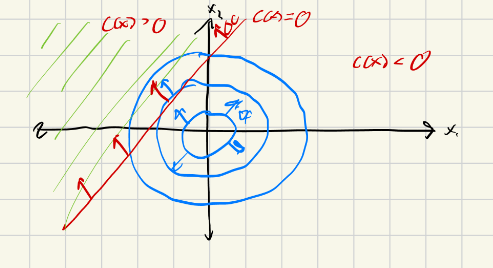
\includegraphics[width=0.5\linewidth]{lecture_5_1.png}
    \end{figure}
    \item Unlike equality case, we can't directly solve KKT conditions with Newton's method
    \item Lots of solution methods:
    \begin{itemize}
        \item Active Set:
        \begin{itemize}
            \item Switch equality constraints on/off and solve inequality constrained problem
            \item Works well if you can guess active set well
        \end{itemize}
        \item Penalty Method
        \begin{itemize}
            \item Replace constraints with cost terms that penalize violation:
            \begin{align*}
                \text{min}_x f(x) 
                \\
                s.t. \quad c(x)\geq 0
                \\
                \text{min}_x f(x) + \frac{\rho}{2}[min(0,c(x)]^2
            \end{align*}
            %insert figure here
            \begin{figure}[H]
                \centering
                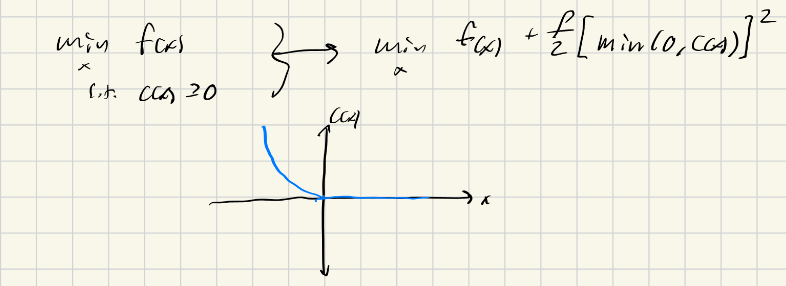
\includegraphics[width=0.75\linewidth]{lecture_5_2.png}
            \end{figure}
            \item Easy to implement
            \item Has issues with ill-conditioning (have to crank $\rho\rightarrow\infty$
            \item Can't solve to high accuracy
            \item Popular fix: estimate $\lambda$ from penalty at each iteration $\rightarrow$ converge with finite $\rho$. Called ``Augmented Lagrangian" (Also closely related ADMM)
        \end{itemize}
        \item Interior Point/Barrier Methods
        \begin{itemize}
            \item Replace inequalities with barrier function in objective 
            \begin{align*}
                \text{min}_x f(x)
                \\
                s.t. \quad x\geq 0
                \\
                \text{min}_x f(x) - \rho \log(x)
            \end{align*}
            %insert figure here
            \begin{figure}[H]
                \centering
                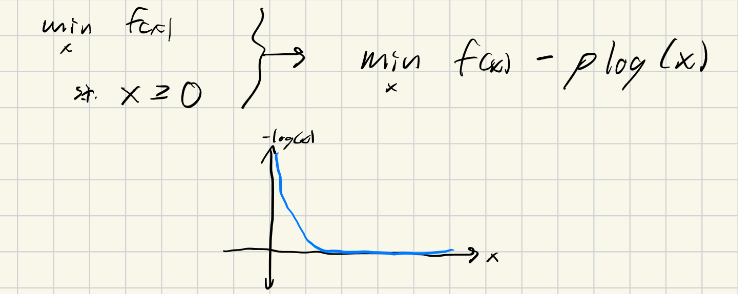
\includegraphics[width=0.75\linewidth]{lecture_5_3.png}
            \end{figure}
            \item Gold standard for convex problems
            \item Fast convergence with Newton
            \item Strong theoretical properties
            \item Used in IPOPT
        \end{itemize}
    \end{itemize}
\end{itemize}

\subsection{Primal Dual Interior Point Method}
\begin{align*}
    \text{min} f(x) \\
    s.t. \quad x&\geq 0
    \\
    &\text{min}_x f(x) - \rho \log(x) 
    \\
    \frac{\partial f}{\partial x} - \frac{\rho}{x} &= 0
\end{align*}
\begin{itemize}
    \item This ``primal" FON condition blows up as $x\rightarrow 0$
    \item we can fix this with the ``primal-dual trick"
    \item Introduce new variable $\lambda=\frac{\rho}{x}\Rightarrow x\lambda = \rho$
    \begin{align*}
        \Rightarrow \nabla f - \lambda &= 0
        \\
        x\lambda &= \rho \quad \text{relaxed complementarity from KKT}
    \end{align*}
    \item Converges to exact KKT solution as $\rho\rightarrow0$. We lower gradually as solver converges from $\rho\approx1$ to $\rho\approx 10^{-8}$
    \item Note we still need to enforce $x\geq 0$ and $\lambda\geq0$ (with linesearch)
    \item We will use another approach ` Log-domain interior point methods for convex optimization"
\end{itemize}

\subsection{Log-Domain Interior Point Method}
\begin{itemize}
    \item More general case:
    \begin{align*}
        \text{min}_x f(x) 
        \\
        s.t. \quad c(x) \geq0
    \end{align*}
    \item Simplify by introducing a ``slack variable"
    \begin{align*}
        \text{min}_{x,s} f(x)
        \\
        s.t. \quad c(x) - s &= 0
        \\
        s&\geq0
        \\
        \text{min}_{x,s} \quad f(x) - \rho\log(s)
        \\
        s.t. \quad c(x)-s &= 0
    \end{align*}
    \item Lagrangian:
    \begin{align*}
        L(x,s,\lambda) &= f(x) - \rho \log(s) - \lambda^T(c(x)-s)
    \end{align*}
    \item FON (first order necessary) Conditions:
    \begin{align*}
        \nabla_xL &= \nabla f - \left(\frac{\partial c}{\partial x}\right)^T\lambda =0
        \\
        \nabla_sL &= \frac{-\rho}{s} + \lambda = 0 \Rightarrow s\circ \lambda = \rho \quad \text{relaxed complementarity}
        \\
        \nabla_\lambda L &= s- c(x) = 0
    \end{align*}
    \item To ensure $s\geq0$ and $\lambda\geq 0$, introduce change of variables:
    \begin{align*}
        s &= \sqrt{\rho}\text{e}^\sigma \Rightarrow \lambda = \sqrt{\rho}\text{e}^{-\sigma}
    \end{align*}
    \item Now (relaxed) complementarity is always satisfied
    \item Plug back into FON conditions:
    \begin{align*}
        \nabla f - \left(\frac{\partial c}{\partial x}\right)^T\sqrt{\rho}\text{e}^{-\sigma} &= 0
        \\
        c(x) - \sqrt{\rho}\text{e}^\sigma &= 0
    \end{align*}
    \item We can solve these with (Gauss) Newton:
    \begin{align*}
        \begin{bmatrix}
            H & \sqrt{\rho}C^T\text{e}^{-\sigma} \\
            C & -\sqrt{\rho}\text{e}^{\sigma} 
        \end{bmatrix}
        \begin{bmatrix}
            \Delta x \\
            \Delta \sigma
        \end{bmatrix}
        &= 
        \begin{bmatrix}
            -\nabla f + C^T \sqrt{\rho}\text{e}^{-\sigma} \\
            -c(x) + \sqrt{\rho}\text{e}^\sigma        
        \end{bmatrix}
    \end{align*}
    \item Example: Quadratic Program
    \begin{align*}
        \text{min}_x \frac{1}{2}x^T Qx + q^T x, \quad Q>0
        \\
        s.t.  \quad Ax &\geq 0
        \\
        Cx &= D
    \end{align*}
    \item Super usefel in control
    \item Can be solved very fast ($\sim$kHz)
\end{itemize}

\end{document}
